\section{Introduction}
Large Language Models (LLMs) have extremely powerful abilities to answer questions or summarize or explain content. However, hallucinations have emerged as a persistent problem, where plausible-looking but incorrect information is mixed in with the generations. Hallucinations create major difficulties for both human users and tool calling or agentic applications due to their visual plausibility, as verifying all portions of the model generation is often just as hard as finding the answer using legacy methods. 

A key challenge is detecting hallucinations in black-box scenarios, where we can access only an LLM's outputs but not its intermediate states—an especially relevant concern when using closed-source commercial APIs. An important intuition is that \emph{self-consistency}—mutual entailment between multiple stochastically sampled high-temperature generations from the LLM for the same question—is lower when the model is hallucinating compared to when it provides a correct answer. As Tolstoy wrote in \emph{Anna Karenina}, ``All happy families are alike; every unhappy family is unhappy in its own way.'' Mechanistically, this LLM behavior can be understood as follows, from the fact that LLMs are pretrained as \emph{statistical} language models. If the model confidently knows the answer, then probability should be concentrated on that answer. If, on the other hand, the model does not know all or part of the answer, its statistical pretraining will bias it towards creating what is essentially a posterior distribution on answers or parts of answers that seem plausible.\looseness=-1

Following this philosophy, prior work \cite{manakul2023selfcheckgpt,farquhar2024detecting,kuhn2023semantic,lin2023generating,nikitin2024kernel} has proposed various methods that leverage self-consistency. However, it remains unclear how much further they can be improved. Thus, we investigate whether we are already near the performance ceiling, given the limited information available in a black-box setting. Using a unified formalization of self-consistency-based methods, we design a method that trains graph neural networks to approximate the ceiling performance of this method family. Notably, we find that existing methods are already close to this ceiling, suggesting little room for further improvement within this paradigm.\looseness=-1



\begin{figure}[!t]
\centering
 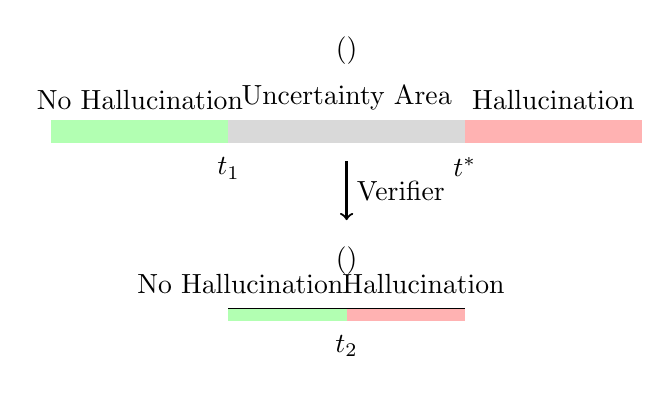
\begin{tikzpicture}[scale=0.75]
    % Stage 1: Real line with t_1 and t_*
    \draw[thick] (0, 0) -- (10, 0); % Real line

    % Label for Stage 1
    \node[above=10pt] at (5, 0.5) {$\mpd(\mself)$};

    % Points t_1 and t_*
    \node[below=6pt] at (3, 0) {$t_1$};
    \node[below=6pt] at (7, 0) {$t^*$};

    % Green shading below t_1
    \fill[green!30] (0, -0.2) rectangle (3, 0.2);
    \node[above] at (1.5, 0.2) {No Hallucination};

    % Gray shading between t_1 and t_*
    \fill[gray!30] (3, -0.2) rectangle (7, 0.2);
    \node[above] at (5, 0.2) { Uncertainty Area};

    % Red shading above t_*
    \fill[red!30] (7, -0.2) rectangle (10, 0.2);
    \node[above] at (8.5, 0.2) {Hallucination};

    % Arrow from [t_1, t_*] to Stage 2
    \draw[thick, ->] (5, -0.5) -- (5, -1.5) node[midway, right] {Verifier};

    % Label for Cross-Consistency
    \node[below=6pt] at (5, -1.5) {$\mpd(\mcross)$};

    % Stage 2: Real line with t_2
    \draw[thick] (3, -3) -- (7, -3); % Real line

    % Point t_2
    \node[below=6pt] at (5, -3) {$t_2$};

    % Green shading below t_2
    \fill[green!30] (3, -3.2) rectangle (5, -3.0);
    \node[above=2pt] at (3.2, -3) {No Hallucination};

    % Red shading above t_2
    \fill[red!30] (5, -3.2) rectangle (7, -3.0);
    \node[above=2pt] at (6.3, -3) {Hallucination};
\end{tikzpicture}
\vspace{-.1cm}
\caption{ Two Stage Hallucination Detection. First, the self-consistency matrix $\mself$ is formed and the test statistic is computed. This is thresholded with two thresholds, where medium values (gray region) advance to the second stage for disambiguation. The $\mcross$ cross-consistency matrix and test statistic are then computed for these ambiguous samples for final classification. \looseness=-1}
\label{fig: illustration}
\vspace{-.4cm}
\end{figure}


This highlights the need to go beyond self-consistency alone. Thus, we consider the case where an additional model serves as a verifier, and we incorporate consistency checking between answers generated by the target model and the verifier. This approach provides information that self-consistency alone cannot capture. For example, agreement between the two models increases confidence in a response's correctness, while disagreement suggests that at least one model is likely hallucinating. Through experiments, we observe a significant gain in the approximated ceiling performance when both self-consistency and cross-model consistency are taken into account, interestingly, even when the verifier is weaker than the target model. Additionally, we find that linearly combining self-consistency with cross-model consistency can achieve performance very close to this ceiling.

Finally, we address the computational overhead introduced by the verifier model. We propose a budget-aware method that performs cross-model consistency checking for only a specified fraction of questions, keeping the computation budget controllable. This method consists of two stages (illustrated in Fig. \ref{fig: illustration}): first, it performs self-consistency checking; then, it selectively applies cross-model consistency checking only when self-consistency falls in a middle range, where judgment is less reliable. We provide a geometric interpretation of this approach through the lens of kernel mean embeddings, offering theoretical insights into its effectiveness. Through extensive experiments across three datasets and 20 target-verifier combinations, we demonstrate that this adaptive mechanism can achieve high detection performance while significantly reducing computational costs. Additionally, we provide practical suggestions on selecting verifier models based on different budget constraints.\looseness=-1

% Large Language Models (LLMs) have extremely powerful abilities to answer questions or summarize or explain content. However, hallucinations have emerged as a persistent problem, where plausible-looking but incorrect information is mixed in with the generations. Hallucinations create major difficulties for both human users and tool calling or agentic applications due to their visual plausibility, as verifying all portions of the model generation is often just as hard as finding the answer using legacy methods. 

% Entailment-based black-box hallucination detectors seek to detect these hallucinations by sampling multiple high-temperature generations from the language model, applying an entailment classifier to pairs of these samples, and learning a classifier based on these entailments to predict whether the low-temperature model generation is correct \cite{farquhar2024detecting}. 
% These detectors are grounded in the intuition that incorrect answers, or hallucinations, tend to tend to be created at random from the model in settings where it does not know the correct answer, and therefore the set of hallucinated generations have less entailment (higher semantic entropy) than generations where the model confidently knows the answer \cite{farquhar2024detecting, kossen2024semantic}. As Tolstoy wrote in \emph{Anna Karenina}, ``All happy families are alike; every unhappy family is unhappy in its own way.'' Mechanistically, this LLM behavior can be understood as follows, from the fact that LLMs are pretrained as \emph{statistical} language models. If the model confidently knows the answer, then probability should be concentrated on that answer. If, on the other hand, the model does not know all or part of the answer, its statistical pretraining will bias it towards creating what is essentially a posterior distribution on answers or parts of answers that seem plausible. Indeed, this behavior is crucial for creative writing, but when it comes to question answering, this creates randomness in the generation. This behavior is often carefully mitigated by design during post-training, but can still occur in many language models \cite{manakul2023selfcheckgpt,farquhar2024detecting,kuhn2023semantic,lin2023generating,nikitin2024kernel}.      %This perspective parallels the notion that correct model outputs are often consistent and coherent, while hallucinations are more likely to arise unpredictably, reflecting a breakdown in the model's reasoning or knowledge.

% \yx{maybe we can also mention the contributions of Section 3}

% While the above philosophy has been effective for many entailment-based hallucination detection methods, it suffers from fundamental limitations when applied in a single-stage framework. Specifically, two types of errors emerge that are difficult to address with self-consistency alone:
% \begin{itemize}[leftmargin=*]
%     \item \textbf{Low-Entropy Incorrectness:} In cases where the language model demonstrates low entropy (i.e., high mean entailment), a single-stage approach is prone to false negatives. For instance, the model may confidently generate incorrect outputs due to systematic biases or learned misconceptions. Such errors are particularly challenging to detect because they lack the "randomness" typically associated with hallucinations.
%     \item \textbf{Varying Ground-Truth Entropies:} Different tasks or queries inherently possess varying levels of uncertainty in their correct answers. For example, the question ``What is 2 + 2?'' has a deterministic ground truth, while ``What is a random number from 1 to 10?'' inherently encompasses a wide range of valid answers. Single-stage detectors struggle to accommodate this variability, as setting a universal threshold for hallucination detection is inherently limiting.
% \end{itemize}

% Introducing a second-stage model, which we term a \emph{verifier}, can address these challenges by leveraging cross-consistency to refine the predictions of the first stage. A verifier model, particularly when it differs in architecture, training data, or objective from the first-stage model, provides a complementary perspective that enhances the detection process. This improvement can occur in two key ways:
% \begin{itemize}[leftmargin=*]
%     \item \textbf{Identifying Low-Entropy Incorrectness:} A diverse verifier model introduces additional variability that can expose systematic biases or incorrect outputs in the first-stage model. If the verifier's outputs differ substantially from those of the first stage, it signals a higher likelihood of hallucination. Conversely, agreement between the two models lends additional confidence in the correctness of the response.
%     \item \textbf{Correcting for Answer Ambiguity:} In cases where the ground truth allows for a diverse set of valid answers, the verifier model can help capture the underlying clusters of correct responses. By generating outputs that complement those of the first stage, the verifier can mitigate the effects of setting a single, rigid threshold for detection.
% \end{itemize}

% Even when the verifier model is relatively weak, its value lies in introducing diversity—both in terms of reasoning pathways and semantic perspectives. This diversity, combined with cross-consistency, enables a more robust detection of hallucinations by leveraging the complementary strengths of multiple models. 

% In this paper, we empirically validate the benefits of this two-stage approach to hallucination detection. We show that incorporating a verifier model improves detection accuracy while addressing the aforementioned limitations of single-stage methods. Additionally, we propose a budget-friendly, unsupervised variant of this approach that uses the verifier selectively based on uncertainty thresholds in the first stage, highlighted in Figure \ref{fig: illustration}. This adaptive mechanism achieves high detection performance while significantly reducing computational costs. Finally, we provide a geometric interpretation of consistency-based hallucination detection through the lens of kernel mean embeddings, offering theoretical insights into the efficacy of the proposed methods.

\section{Related Work}

There are works that explore white-box detection methods, such as \cite{duan2024shifting,varshney2023stitch}, which require token-level logits, or \cite{yin2024characterizing,zou2023representation,agrawal2023language}, which rely on intermediate representations. White-box methods are less suitable for certain scenarios, such as closed-source commercial APIs. In this work, we focus exclusively on black-box hallucination detection, where we do not have access to the internal workings of the LLM. In this scenario, the primary approach involves checking the consistency between multiple samples of the LLM's answers \cite{manakul2023selfcheckgpt,farquhar2024detecting,kuhn2023semantic,lin2023generating,nikitin2024kernel}. These works rely on sampling multiple answers to the same question from the LLM and using an NLI (Natural Language Inference) model to determine whether they are semantically equivalent. The NLI judgments are then processed in various ways to decide whether a hallucination has occurred. Details of these methods are discussed in Section \ref{sec:3}. \citet{manakul2023selfcheckgpt,kuhn2023semantic} also explore alternative methods for judging semantic equivalence, which are either less effective (e.g., n-gram) or computationally expensive (e.g., using an LLM). \cite{SAC3_hallucination_detection_black_box_lms} identify limitations in self-consistency-based methods and propose leveraging question perturbation and cross-model response consistency (comparing an LLM's responses with those from an additional verifier LLM) to improve performance. While their approach improves results, introducing a verifier model adds computational overhead. In this work, we systematically explore the possibility of achieving computational efficiency when combining self-consistency and cross-model consistency. Note that the question perturbation technique from \cite{SAC3_hallucination_detection_black_box_lms} is orthogonal to our approach and could potentially be incorporated to achieve better results. Another line of work involves directly asking LLMs to judge the uncertainty of their answers \cite{mielke2022reducing,tian2023just,kadavath2022language,lin2022teaching}, which typically requires additional finetuning/calibration and does not fit within the black-box scenario. Without any modification to the original LLMs, their verbalized confidence is often inaccurate \cite{xiong2023can}. The inherent conflict between calibration and hallucination, as theoretically shown in \cite{calibrated_language_models_must_hallucinate}, further highlights the limitations of this approach. There are also works addressing hallucination mitigation, such as using RAG \cite{asai2023self,gao2022rarr}, inference-time intervention \cite{li2024inference}, or fine-tuning \cite{lee2022factuality,tian2023fine}, which is beyond the scope of this paper.\looseness=-1



\section{Preliminaries}

In the task of hallucination detection, we have a target LLM, denoted by $\gM_t$, for which we aim to detect hallucinations.  We are given a set of questions $\{q_i\}_{i=1}^n$. Given a set of questions $\{q_i\}_{i=1}^n$, the model generates answers, $a_i\! =\! \gM_t(q_i, \tau)$, under a specified temperature $\tau$. The ground truth annotation $\hat{h}_i$ indicates whether $a_i$ is a hallucination ($\hat{h}_i = 1$) or factual ($\hat{h}_i = 0$).  The objective is to predict whether $a_i$ is a hallucination, with our prediction denoted by $h_i$. \looseness=-1

To achieve this, many methods are designed to output a value, $v_i$, that captures specific characteristics (e.g., the uncertainty of the answer). A higher value of $v_i$ suggests that $a_i$ is more likely to be a hallucination. The prediction $h_i$ is then determined based on a threshold applied to $v_i$, where the choice of threshold dictates the final classification.

To evaluate the performance of a hallucination detection method, we focus on two widely accepted metrics computed given outputs $\{v_i\}_{i=1}^n$ and ground truths $\{\hat{h}_i\}_{i=1}^n$: (1) \textbf{AUROC}, area under the receiver operating characteristic curve. is a classic performance measure in binary classification. It captures the trade-off between the true positive rate and the false positive rate across various thresholds, providing an aggregate measure of the model's ability to distinguish between the two classes. (2) \textbf{AURAC}, the area under the ``rejection accuracy'' curve \cite{farquhar2024detecting}. It is designed for scenarios where a hallucination detection method is employed to refuse answering questions that the model is most likely to hallucinate on. Rejection accuracy measures the model's accuracy on the $X$\% of questions with the lowest $v_i$ values (least likely to hallucinate), and the area under this curve summarizes performance across all values of $X$.\looseness=-1
\vspace{-.2cm}

\section{From Self-consistency to Cross-Consistency}
\label{sec:3}
\begin{figure*}[!t]
    \centering
    \subfigure[\llamatwothirteen  \label{}]{
        \includegraphics[width=0.3\textwidth]{figures/method_vs_gcn/squad/meta-llama_llama-2-13b-chat_auroc.pdf}
    }
    \subfigure[ \llamathreeseventy \label{}]{
        \includegraphics[width=0.3\textwidth]{figures/method_vs_gcn/squad/meta-llama_llama-3-70b-instruct_auroc.pdf}
    }
    % Third subfigure
    \subfigure[ \mixtral \label{}]{
        \includegraphics[width=0.3\textwidth]{figures/method_vs_gcn/squad/mistralai_mixtral-8x7b-instruct-v01_auroc.pdf}
    }

\vspace{-.2cm}
    \subfigure[\llamatwothirteen\label{}]{
        \includegraphics[width=0.3\textwidth]{figures/method_vs_gcn/triviaqa/meta-llama_llama-2-13b-chat_auroc.pdf}
    }
    \subfigure[\llamathreeseventy\label{}]{
        \includegraphics[width=0.3\textwidth]{figures/method_vs_gcn/triviaqa/meta-llama_llama-3-70b-instruct_auroc.pdf}
    }
    % Third subfigure
    \subfigure[\mixtral\label{}]{
        \includegraphics[width=0.3\textwidth]{figures/method_vs_gcn/triviaqa/mistralai_mixtral-8x7b-instruct-v01_auroc.pdf}
    }
    \vspace{-.2cm}
    \caption{Comparison between AUROC of existing methods and the approximated ceiling performance on SQuAD ((a)–(c)) and TriviaQA ((d)–(f)). We observe that, across all setups, the best method performs very close to the oracle, indicating that we are approaching the performance limit. A similar result is observed for AURAC in Fig. \ref{fig: methods_vs_gcn_rac}.}
    \label{fig: methods_vs_gcn_roc}
    \vspace{-.1cm}
\end{figure*}

\subsection{Self-consistency based detection}\label{subsec: approx_ceiling_self}

Prior work \cite{manakul2023selfcheckgpt,farquhar2024detecting,kuhn2023semantic,lin2023generating,nikitin2024kernel} has introduced various methods leveraging self-consistency. However, the extent to which these methods can be further improved remains unclear. To explore this, we develop a method to approximate the ceiling performance for any approach that utilizes self-consistency and compare it against the performance of existing methods.

%Recent work has focused on detecting hallucinations in LLMs' responses by analyzing uncertainty. In particular, recent studies have highlighted the importance of semantic uncertainty, measured via semantic entropy \cite{kuhn2023semantic,farquhar2024detecting}. Semantic entropy has shown promise in distinguishing hallucinations from factual outputs and has outperformed earlier methods of uncertainty measurement. Notably, it can be estimated in a black-box manner, i.e., without access to any intermediate outputs of LLMs. Building on these findings, subsequent black-box detection techniques \cite{lin2023generating,nikitin2024kernel} have been proposed to further refine semantic entropy, introducing more fine-grained and sophisticated approaches.

% An important question arises: how far are we from the performance ceiling? Are we already approaching the limit, given the minimal information available in the black-box scenario? To address this, we design a method to approximate the ceiling performance and compare it against the performance of existing methods.

% \subsubsection{Approximating the ceiling performance}\label{subsec: approx_ceiling_self}

\textbf{Unified formalization of self-consistency-based methods.} We first present a unified formalization of the existing methods. Recall that the goal is to determine whether each $\gM(q_i)$ is a hallucination. All these methods rely on additionally sampling $m$ answers from the LLM $\gM$ for question $q_i$ under a high temperature $\tau'$, which is typically much higher than $\tau$, the temperature used to generate $a_i$. For example, in \cite{farquhar2024detecting}, the settings are $\tau = 0.1$ and $\tau' = 1.0$. Let $\{a'_{i,j}\}_{j=1}^{m}$ denote the set of these additionally sampled answers. These methods then use an entailment estimator (e.g., \texttt{DeBERTa-Large-MNLI}), denoted by $\gE$. The estimator $\gE$ takes two answers as input and outputs a value between 0 and 1, indicating the degree of entailment between the two answers, where 1 means full entailment. Using $\gE$, a self-entailment matrix $\mself_i$ is constructed as: $
    \mself_i = [ \gE( a'_{i, j}, a'_{i, k} )  ]_{1\leq j\leq m, 1\leq k\leq m} $,
where each element is the entailment value for a pair of answers in $\{a_{i,j}'\}_{j=1}^m$. Existing methods can then be formalized as some function $f$ applied to the self-entailment matrix $\mself_i$ which outputs a scalar. The focus of prior work lies in designing various forms of 
$f$. Specifically, (1) $\se(\mself)$, the Semantic Entropy \cite{farquhar2024detecting}, uses a binarized version of $\mself_i$ to identify which answers belong to the same semantic set and then computes the entropy over these semantic sets. (2) $\mpd(\mself_i)$ \cite{lin2023generating,manakul2023selfcheckgpt} is simply the mean pairwise distance, computed as $1 - \text{Mean}(\mself_i)$. (3) $\eigv(\mself_i)$ \cite{lin2023generating} is defined as the sum of the eigenvalues of the graph Laplacian of $\mself_i$. (4) $\ecc(\mself_i)$ \cite{lin2023generating} measures the eccentricity of the answers leveraging the eigenvectors of the graph Laplacian of $\mself_i$. (5) $\kle(\mself_i)$, the Kernel Language Entropy \cite{nikitin2024kernel}, involves applying the von Neumann entropy to a graph kernel derived from $\mself_i$.
For all these methods, a higher output indicates greater uncertainty among $\{a_{i,j}'\}_{j=1}^m$, making the corresponding low-temperature answer $a_i$ more likely to be a hallucination. \looseness=-1

The underlying assumption is that $\mself_i$ contains exploitable information related to $\hat{h}_i$, the ground truth hallucination annotation. This prompts the question: how much information does $\mself$ actually encode about $\hat{h}_i$? To explore this, we aim to identify the optimal function $f$ that maps $\mself$ to the hallucination label. This leads to the following formulation:
\vspace{-.2cm}
\begin{equation}
\label{eq: loss_gcn}
   \hat{f} = \argmin_{f} \E[l(f(\mself), \hat{h})],    
\end{equation}
where \(l\) is a loss function that measures the discrepancy between the output value and the actual label. 

\textbf{Approximating the ceiling performance with GCN models.} To search for $\hat{f}$, we frame it as a learning problem. Since the task is ultimately binary classification based on the matrix $\mself$, graph neural networks are well-suited due to their ability to process matrix structures and express a wide range of functions. We use a two-layer Graph Convolutional Network (GCN) to represent $f$. The model is trained with BCE loss on sampled pairs of $\mself$ and $\hat{h}$. We then evaluate AUROC and AURAC of the resulting model as an approximation of the ceiling performance. The training and test samples are drawn independently to account for the finiteness of the data, ensuring that the evaluation reflects the model's ability of capturing a generalizable relationship between $\mself$ and $\hat{h}$, rather than that of overfitting the training data. \looseness=-1

%\subsubsection{results} 
\textbf{Results.} In Figs. \ref{fig: methods_vs_gcn_roc} and \ref{fig: methods_vs_gcn_rac}, we compare the performance of existing methods with the ceiling performance approximated using the aforementioned approach across various settings. We consider three different LLMs: \llamatwothirteen{}, \llamathreeseventy{}, and \mixtral{}, as well as two datasets: SQuAD and TriviaQA. In the plots, the x-axis represents different methods with varying hyperparameters. The best-performing method varies across different settings, with \mpd{}, \kle{}, and \eigv{} consistently showing relatively strong performance. Notably, in each setting, the top method closely approaches the approximated ceiling, indicating that existing methods already make near-maximal use of $\mself$, particularly when sufficient validation data is available to optimize method and hyperparameter selection.
%(2) There is still potential for improvement in developing a more robust method that consistently approaches ceiling performance without requiring extensive hyperparameter tuning or one that is less sensitive to hyperparameter choices. Achieving this, however, could be highly challenging, as different settings (e.g., combinations of models and datasets) may demand tailored approaches. 
\looseness=-1

\begin{figure*}[!t]
    \centering
    \includegraphics[width=0.99\linewidth]{figures/w_and_wo_cross/w_and_wo_cross.pdf}
    \vspace{-.2cm}
    \caption{Comparison between approximated ceiling performances using only $\mself$ (gray) and those using both $\mself$ and $\mcross$. The x-axis shows the target model, and the colors indicate the verifier model, as shown in the legend. We observe a clear improvement when a verifier model is used, in terms of both AUROC and AURAC.\looseness=-1}
    \label{fig: w_and_wo_cross}
    \vspace{-.3cm}
\end{figure*}

\subsection{Incorporating cross-model consistency}

As noted in the previous subsection, existing methods bring us very close to the ceiling performance for self-consistency alone. The question now is: how can we push beyond this limit? In the black-box scenario, our options are constrained by the lack of access to any internal model information. \cite{SAC3_hallucination_detection_black_box_lms} has explored another potential approach: leveraging outputs from other LLMs to improve hallucination detection through cross-model comparisons. A minimal case involves using one additional model as a verifier. This added layer of information can help further refine hallucination detection. For example, if two models significantly disagree on their answers, at least one is likely hallucinating.  \looseness=-1

\subsubsection{Improvement in the ceiling performance} \label{sec: improvement_ceiling_cross}
We explore how much gain cross-model consistency checking can possibly bring. Let us denote this verifier model as $\gM_v$. Similar to the self-consistency case, a natural extension is to encode the cross-model consistency information in a matrix: $\mcross_i = [ \gE(a'_{i,j}, b'_{i,k}) ]_{1 \leq j \leq m, 1 \leq k \leq m }$, where $\{ b'_{i,k} \}_{k=1}^m$ are $m$ answers sampled from $\gM_v$ under temperature $\tau'$ for question $q_i$. Thus, $\mcross_i$ captures the pairwise entailment relationships between the answers generated by the target model $\gM_t$ and the verifier model $\gM_v$. 

\begin{remark}[Cross entailment]
To build intuition, consider the setting of a very strong verifier model that always returns a sample from the ground truth distribution. Then, if the entailment model returns a calibrated posterior probability of entailment, it is easy to see that $\mathrm{Mean}(\mcross_i)$ is the probability of entailment between an $\mathcal{M}_t$ sample and a ground truth sample. In other words, it can be interpreted as the probability of correctness. For as the verifier becomes weaker, we hypothesize that the $\mathrm{Mean}(\mcross_i)$ retains significant correlation with the probability of correctness, and observe this in practice.
\end{remark}\looseness=-1

Building on the formalization in Section \ref{subsec: approx_ceiling_self}, we aim to determine how much information can be extracted when both $\mself$ and $\mcross$ are used to predict the ground truth hallucination label. To achieve this, we search for a function $f$ that takes both $\mself$ and $\mcross$ as input. Given the pairwise nature of the data, we again leverage GCN models to represent the function. Specifically, we combine $\mself$ and $\mcross$ into a single matrix: $\begin{bmatrix}
\mself & \mcross\\
\mcross & \mathbf{0}
\end{bmatrix}$
which encodes the underlying structure of the data as pairwise relationships between answers. We then apply a GCN to this combined matrix and train the model to fit the ground truth labels $\hat{h}$. Finally, we evaluate the resulting model to approximate the ceiling performance achievable with both $\mself$ and $\mcross$.

\begin{figure}[!t]
\centering
\includegraphics[width=0.25\linewidth]{figures/weighted_avg/auroc/squad/meta-llama_llama-2-13b-chat/meta-llama_llama-3-70b-instruct/multiple.pdf}
\includegraphics[width=0.25\linewidth]{figures/weighted_avg/auroc/squad/meta-llama_llama-3-70b-instruct/meta-llama_llama-2-13b-chat/multiple.pdf}
\includegraphics[width=0.25\linewidth]{figures/weighted_avg/auroc/squad/mistralai_mixtral-8x7b-instruct-v01/meta-llama_llama-2-13b-chat/multiple.pdf}

\includegraphics[width=0.25\linewidth]{figures/weighted_avg/auroc/squad/meta-llama_llama-2-13b-chat/mistralai_mixtral-8x7b-instruct-v01/multiple.pdf}
\includegraphics[width=0.25\linewidth]{figures/weighted_avg/auroc/squad/meta-llama_llama-3-70b-instruct/mistralai_mixtral-8x7b-instruct-v01/multiple.pdf}
\includegraphics[width=0.25\linewidth]{figures/weighted_avg/auroc/squad/mistralai_mixtral-8x7b-instruct-v01/meta-llama_llama-3-70b-instruct/multiple.pdf}
\vspace{-.2cm}
\caption{A simple weighted average of self-consistency and cross-consistency-based metrics, $(1-\lambda) \mpd(\mself) + \lambda \mpd(\mcross)$, can achieve performance close to that of the oracle method. Plots for AURAC are in Fig. \ref{fig: weighted_avg_aurac} in Appx. \ref{apdx: additional_exp}.\looseness=-1
}
\label{fig: weighted_avg}
\vspace{-.3cm}
\end{figure}

We now compare the approximated ceiling performances achieved using only $\mself$ to those achieved using both $\mself$ and $\mcross$, as shown in Fig. \ref{fig: w_and_wo_cross}. The x-axis represents the target model, while the colors indicate the verifier model used. Gray bars correspond to the scenario where only $\mself$ is used, i.e., no verifier model is involved. The results demonstrate a clear improvement in performance, measured by both AUROC and AURAC, when a verifier model is introduced. Interestingly, this improvement is observed even in cases where the target model itself is quite strong. For example, on the TriviaQA dataset, adding a weaker verifier model can still enhance detection performance when \llamathreeseventy{} is used as the target model. This highlights the potential of leveraging cross-model consistency, as even a less powerful verifier can provide complementary insights that enhance hallucination detection.\looseness=-1


\subsubsection{Linearly combining MDPs closely approaches the ceiling}\label{sec:weighting}


Although the function the GCN implements to achieve ceiling performance is unknown, interestingly, we find that a simple extension of existing methods can perform almost equally well. We leverage \mpd{} introduced earlier, which can be naturally extended to $\mcross$ as $\mpd(\mcross) = 1 \!- \!\text{Mean}(\mcross)$. The combined approach uses a weighted average: $(1-\lambda) \mpd(\mself) + \lambda \mpd(\mcross)$, where $\lambda$ is a hyperparameter. As shown in Fig. \ref{fig: weighted_avg}, with an appropriate choice of $\lambda$, this method achieves performance very close to the approximated ceiling performance. \looseness=-1

% \todoblue{adjust the above accordingly and add the theory  after finalizing the theory} %\ym{should we talk about this only in appendix ?}


\section{Budget-Aware Hallucination Detection with A Verifier Model  }\label{sec: method}

% Actor/Verifier

%\todoblue{shall we place "target" with "actor" everywhere else}\ym{replaced actor by target}

% \begin{algorithm}[!t]
%    \caption{Budget-aware two-stage detection}
%    \label{alg: two_stage}
%    \small
% \begin{algorithmic}
%    \STATE {\bfseries Input:} questions $\{q_i\}_{i=1}^n$, target model $\gM_\tar$, verifier model $\gM_\ver$, number of samples $m$, temperature $\tau'$, entailment estimator $\gE$, %fraction of questions sent to the verifier  $p$, 
%    thresholds $t_1, t_2, t^\ast$
%    \STATE {\bfseries Output:} indicators of whether $\gM_\tar$ hallucinates for each given question $\{h_i\}_{i=1}^n$
%    \FOR{$i=1$ {\bfseries to} $n$}
%    \STATE $\{a_{i, j}'\}_{j=1}^{m} \leftarrow$ the $m$ responses sampled from $\gM_\tar$ for the question $q_i$ under temperature $\tau'$
%    \STATE $\mself_i \leftarrow [\gE( a_{i,j}', a_{i,k}')]_{1\leq j\leq m, 1\leq k \leq m }$ 
%    \STATE $\sself_i\leftarrow \mpd(\mself_i) $
%    \ENDFOR
%    %\STATE $t^* \leftarrow \text{s.t. $pn$ elements in $\{\sself_i\}_{i=1}^n$ fall within $[t_1, t^*]$}  $
%    \FOR{$i=1$ {\bfseries to} $n$}
%    \IF{$\sself_i\in [t_1, t^*]$}
%    \STATE $\{b_{i,j}'\}_{i=1}^{m} \leftarrow$ the $m$ responses sampled from $\gM_\ver$ for the question $q_i$ under temperature $\tau'$
%    \STATE $\mcross_i \leftarrow [\gE( a_{i,j}', b_{i,k}')]_{1\leq j\leq m, 1\leq k \leq m }$ 
%    \STATE $\scross_i \leftarrow \mpd(\mcross_i) $
%    \STATE $h_i \leftarrow 0~ \text{if}~ \scross_i< t_2 ~\text{else}~ 1 $
%     \ELSIF{ $\sself_i< t_1$ } 
%     \STATE $h_i \leftarrow 0$
%     \ELSE
%     \STATE $h_i \leftarrow 1$
%    \ENDIF
%    \ENDFOR
% \end{algorithmic}
% \end{algorithm}

\begin{algorithm}[!t]
   \caption{Budget-aware two-stage detection}
   \label{alg: two_stage}
   \small
\begin{algorithmic}
   \STATE {\bfseries Input:} question $q$, target model $\gM_\tar$, verifier model $\gM_\ver$, number of samples $m$, temperature $\tau'$, entailment estimator $\gE$, %fraction of questions sent to the verifier  $p$, 
   thresholds $t_1, t_2, t^\ast$.
   %\STATE {\bfseries Output:} indicator $h$ of whether $\gM_\tar$ hallucinates.
   %\FOR{$i=1$ {\bfseries to} $n$}
   \STATE $\{a_{j}'\}_{j=1}^{m} \leftarrow$ the $m$ responses sampled from $\gM_\tar$ for the question $q$ under temperature $\tau'$ \COMMENT{{\color{darkgreen}First stage}}
   \STATE $\mself \leftarrow [\gE( a_{j}', a_{k}')]_{1\leq j\leq m, 1\leq k \leq m }$ 
   \STATE $\sself\leftarrow \mpd(\mself) $
   %\ENDFOR
   %\STATE $t^* \leftarrow \text{s.t. $pn$ elements in $\{\sself_i\}_{i=1}^n$ fall within $[t_1, t^*]$}  $
   %\FOR{$i=1$ {\bfseries to} $n$}
   \IF{ $\sself< t_1$ } 
   \RETURN $h = \FALSE$ \COMMENT{{\color{darkgreen}no hallucination}}
   \ELSIF{$\sself> t^\ast$}
   \RETURN $h = \TRUE$  \COMMENT{{\color{darkgreen}hallucination}}
   \ELSE %\COMMENT{Advance to second stage}
   \STATE $\{b_{j}'\}_{j=1}^{m} \leftarrow$ the $m$ responses sampled from $\gM_\ver$ for the question $q_i$ under temperature $\tau'$ \COMMENT{{\color{darkgreen}Second stage}}
   \STATE $\mcross \leftarrow [\gE( a_{j}', b_{k}')]_{1\leq j\leq m, 1\leq k \leq m }$ 
   \STATE $\scross \leftarrow \mpd(\mcross) $
   \RETURN $h = \FALSE~ \text{if}~ \scross_i< t_2 ~\text{else}~ \TRUE $
    
   \ENDIF
   %\ENDFOR
\end{algorithmic}
\end{algorithm}


From the previous section, we observe that performance improves significantly when self-consistency checking is combined with cross-model consistency checking. However, this approach can introduce substantial computational overhead, especially when the verifier is a large model. For instance, with a 7B target model and a 70B verifier model, cross-model consistency adds 10 times the computation.

To address this issue, we propose a method to control computational overhead. As illustrated in Fig. \ref{fig: illustration}. The key idea is to perform cross-model consistency checking only when it is most necessary. Intuitively, when self-consistency scores are extremely high or low, it is likely—though not guaranteed—that the model's output is non-hallucinatory or hallucinatory, respectively. In such cases, performing cross-model consistency checking may not be necessary under limited computational budgets. Instead, cross-model consistency should focus on cases with intermediate self-consistency scores, where our judgment is more uncertain. This is formalized in Alg. \ref{alg: two_stage}. The parameter \( p \) specifies the fraction of instances for which cross-model consistency checking will be performed. The parameter \( t_1 \) is the threshold for $\mpd(\mself)$ below which the output is deemed non-hallucinatory. Based on \( t_1 \), we choose to compute \( t^* \), the threshold for $\mpd(\mself)$ above which the output is classified as hallucinatory, such that only \( p \) of the $\mpd(\mself)$ scores fall between \( t_1 \) and \( t^* \). For these intermediate cases, judgments are made based on cross-model consistency $\mpd(\mcross)$ using a threshold \( t_2 \).\footnote{We threshold $\mpd(\mcross)$ directly in the second stage (instead of a linear combination as in Section \ref{sec:weighting}, since (a) it saves a hyperparameter and (b) we are able to approach the GCN-based performance ceiling without it.} Note that we use \( \mpd \) to measure inconsistency from \( \mself \) due to its simplicity, ease of extension to \( \mcross \) (unlike, e.g., \( \kle \), which is specifically designed for \( \mself \) but not immediately well-defined for \( \mcross \)), and the fact that it contains sufficient information for achieving ceiling performance, as discussed in Sec. \ref{sec:weighting}. Future work could explore other metrics.\looseness=-1

% \subsection{Types of 1st-stage errors and how 2nd-stage can correct}


% \textcolor{red}{under which assumptions we have correctness of the algorithm : @yihao ---> claim what are optimal tresholds under the assumptions }

